\section{Projeto de Hardware}

Com base nos requisito, foram determinados os principais componentes do projeto
para o controle e monitoramento do sistema

\subsection{Microcontrolador}

% TODO: Atualizar para Wemos D1
O microcontrolador Arduino Uno R3 é versátil e ideal para a prototipagem e será
utilizado como microcontrolador do projeto. O mesmo possui portas i/o analógicas e
digitais, fontes de alimentação de 3,3V/5V e é programado na linguagem C.

\begin{figure}[h]
    \centering
    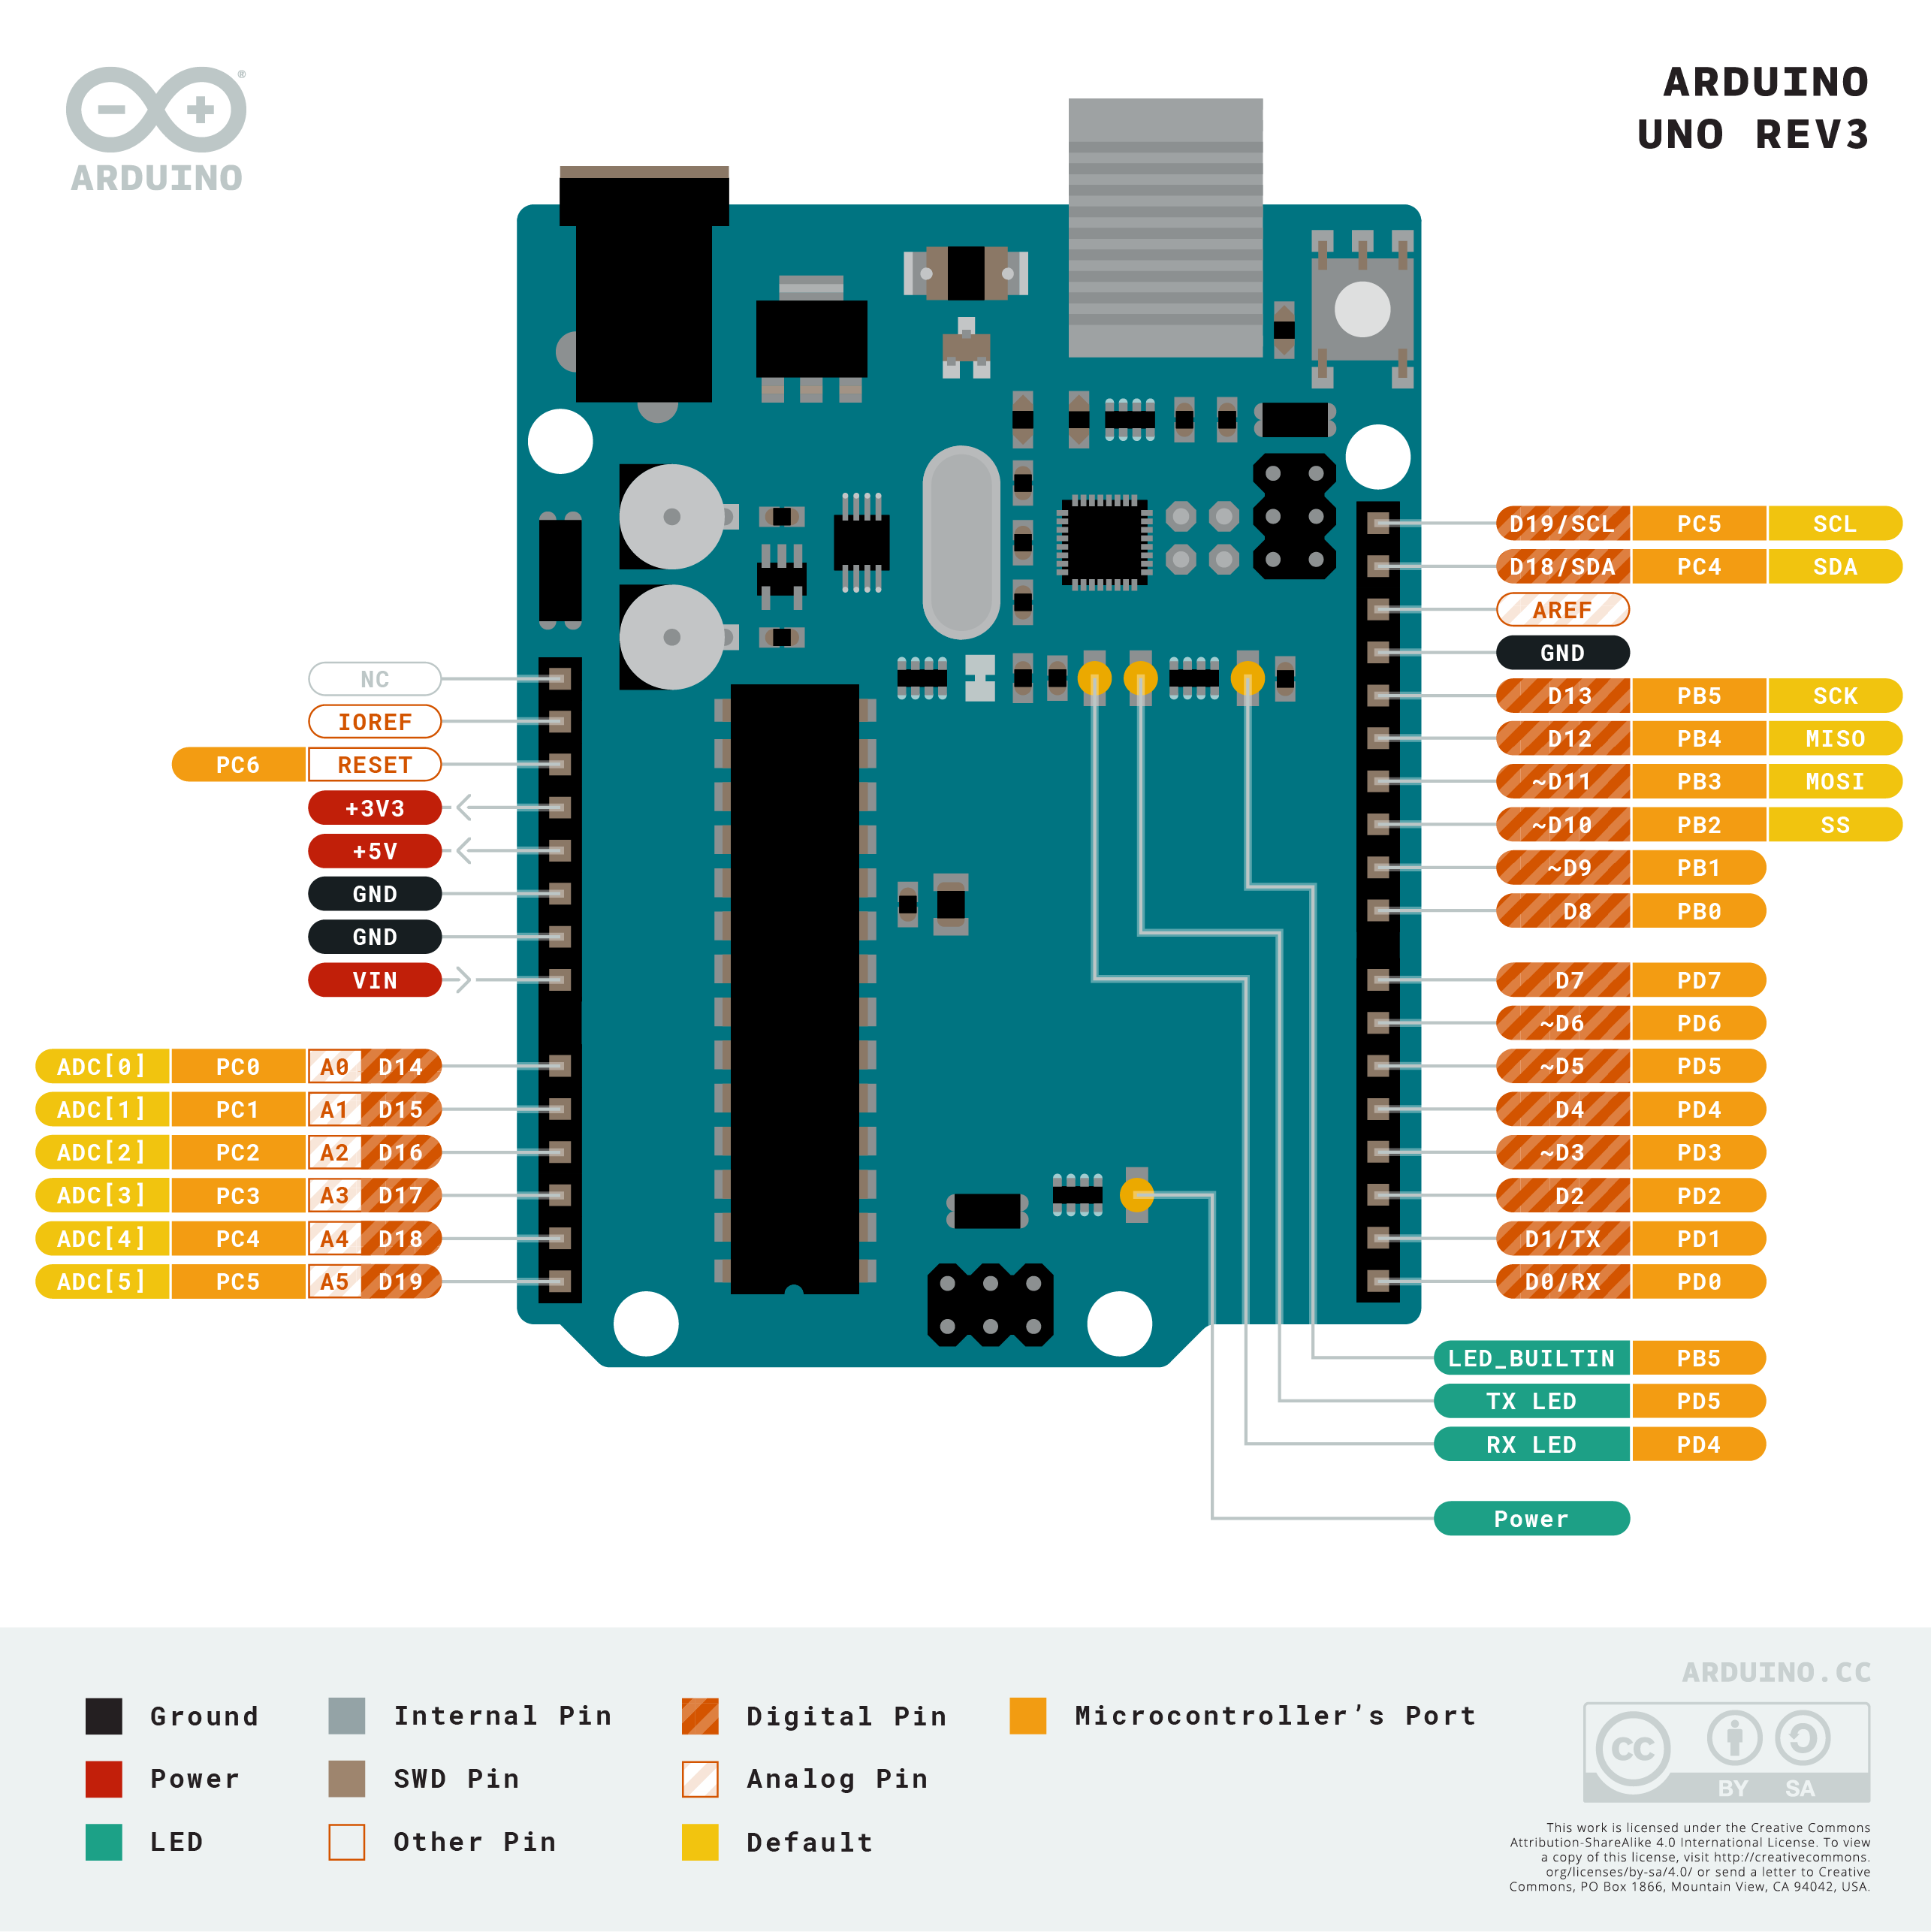
\includegraphics[scale=0.35]{figuras/projeto/hardware/arduino.png}
    \caption{Arduino Uno R3}
    \label{fig:arduino}
\end{figure}

\subsection{Sensores}

A definição dos sensores a serem utilizados se baseou nos seguintes critérios, em ordem de importância:

\begin{itemize}
    \item Faixa de operação compatível com os requisitos e especificidades do sistema
    \item Disponibilidade no mercado brasileiro
    \item Compatibilidade com o Arduino
    \item Custo de aquisição
\end{itemize}

O primeiro critério é trivial, e deve ser eliminatório em qualquer avaliação. O critério de disponibilidade no mercado brasileiro teve essa classificação pelo desejo de se adquirir e trabalhar com os sensores o mais rápido possível e mitigar o risco com atrasos devido a importações e falta de estoque. A compatibilidade com o Arduino exprime quão diretamente um sensor pode ser utilizado, principalmente em relação a alimentação, sendo preferíveis sensores que tenham tensões de entrada em comum com o microcontrolador, i.e., 3,3 ou 5V. Finalmente, custos de aquisição menores são preferíveis.

\subsubsection{Temperatura}

Para a medição de temperatura o sensor escolhido foi o circuito integrado DS18B20 (Figura \ref{fig:ds18b20}) com uma vedação impermeável. É um sensor que atende as especificações e é amplamente utilizado em conjunto com o Arduino e microcontroladores semelhantes, e possui alta disponibilidade no mercado a um baixo custo, sendo comercializado em uma versão impermeável, muita prática para esse projeto. A leitura da temperatura pelo microcontrolador é realizada por apenas um fio de dados, utilizando a interface One-Wire. 

Ficha técnica:
\begin{itemize}
    \item Tensão de operação: 3-5,5V
    \item Faixa de medição: -55°C a +125°C
    \item Precisão: ±0.5°C entre -10°C e +85°C
    \item Ponta de aço inoxidável
\end{itemize}

\begin{figure}[h]
    \centering
    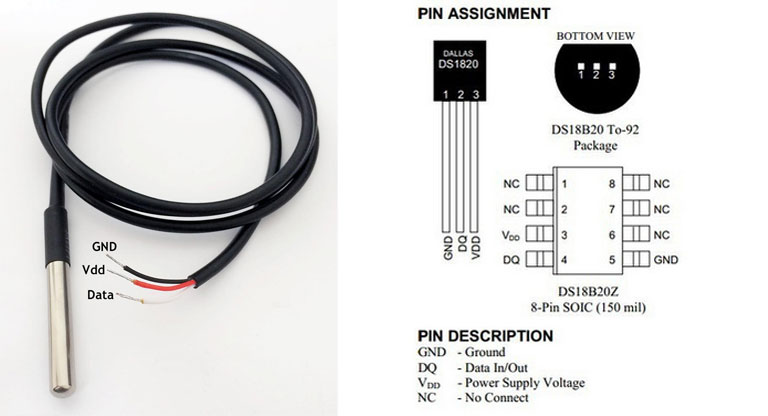
\includegraphics[scale=0.35]{figuras/projeto/hardware/ds18b20.jpg}
    \caption{Sensor DS18B20}
    \label{fig:ds18b20}
\end{figure}

\subsubsection{Densidade Relativa}

A medição da densidade relativa é menos trivial pela ausência de sensores completos comercializados a baixo custo. Quando não é automatizada, a medição é comumente  realizada com auxílio de um densímetro ou um refratômetro, que medem a densidade relativa e a concentração de açúcar dissolvido em graus Brix, respectivamente. Ambas as ferramentas requerem interação humana e a extração de uma pequena amostra da solução, aproximadamente 100 a 250ml e algumas gotas, respectivamente.


% TODO: Referência Boulton e Quain (2001)
Quanto a medição automática e contínua da densidade relativa, Boulton e Quain (2001) apresentam algumas formas de medir a grandeza, destacam-se: a utilização de sensores de pressão posicionados em diferentes alturas do fermentador, e computando a diferença de pressões medidas; e utilizando um sensor ultrassônico,  medindo o tempo que um pulso leva para ser transmitido entre dois pontos fixos, entremeado pela solução. 


Em pesquisa por soluções existentes no mercado, a abordagem de dois produtos são dignas de consideração: o Beer Bug utiliza uma célula de carga para medir o empuxo sofrido por um peso submerso na solução, e o Plaato, que utiliza a medição do gás carbônico expelido durante a fermentação para calcular indiretamente a densidade relativa.


Dentre as opções listadas, a medição por diferença de pressões e empuxo foram selecionadas para serem adotadas em primeiro momento no projeto, com prioridade da primeira. Essas são as soluções que aparentam apresentar menor complexidade na medição e maior facilidade na calibração para obtenção de resultados consistentes.


As opções listadas são discutidas a seguir, contemplando as especificações necessárias para cada sensor, e os modelos escolhidos para utilização no projeto.

\paragraph{Medição por diferença de pressão} 


Esse método se baseia na seguinte relação:

\begin{equation}
P_{estatica} = \rho \cdot g \cdot h
\end{equation}

A pressão estática medida em determinado ponto de um fluido é igual ao produto da densidade  desse fluido, da aceleração gravitacional g, e da altura h da coluna de líquido. Consequentemente, considerando a densidade homogênea e a variação da aceleração gravitacional desprezível, a diferença de pressão entre dois pontos em diferentes alturas desse fluido, é:

\begin{equation}
\Delta P = \rho \cdot g \cdot \Delta h
\end{equation}

Dessa forma, mantendo a diferença de alturas hfixa e conhecida, é simples inferir o valor da densidade a partir da medida da diferença de pressão medida pelo sensor.


Seguindo o requisito HW-F-3, o sistema deve ser capaz de medir densidades relativas de 1,000 e 1,150, em relação à água a 20 °C, o que corresponde a uma faixa entre 998,203 e 1147,933 kg/m³. Considerando a aceleração gravitacional 9.807 m/s² e uma distância de 20 cm entre os dois pontos medidos (o que é razoável para fermentadores pequenos, até 50L), a faixa de operação do sensor de diferencial de pressão deve ser, em diferentes unidades comerciais:

\begin{table}
    \begin{center}
        \begin{tabular}{ |c|c|c|c| } 
            \hline
            Valor / Unidade & N/m² ou Pa & bar & psi \\
            \hline
            Mínimo & 1957,805 & 0,019578 & 0,284 \\ 
            \hline
            Máximo & 2251,476 & 0,022515 & 0,327 \\ 
            \hline
        \end{tabular}
        \caption{\label{tab:densidades}Diferenças de pressão esperadas para cálculo da densidade relativa.}
    \end{center}
\end{table}

Para obter a precisão de 1 milésimo de densidade relativa, o sensor necessita de uma precisão de aproximadamente 0,1\%.


A partir das especificações, foram buscados os sensores disponíveis no mercado, principalmente os produzidos pela Mouser Electronics (https://br.mouser.com/). Seguindo os critérios definidos, o modelo escolhido foi o MPXV7002DP, que possui as seguintes especificações:

\begin{itemize}
\item Faixa de medição: -0.3 a +0.3 psi
\item Precisão: 2,5\%
\item Tensão de alimentação: 5V
\end{itemize}

Apesar do sensor não apresentar uma precisão adequada, acreditamos que o uso da média de diversas medidas e calibração com algumas medidas feitas pelo usuário podem propiciar resultados satisfatórios.

\begin{figure}[h]
    \centering
    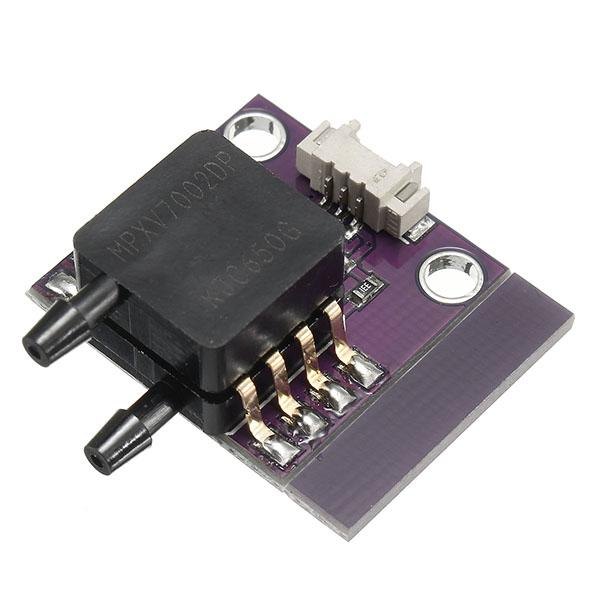
\includegraphics[scale=0.30]{figuras/projeto/hardware/MPXV7002DP.jpg}
    \caption{Sensor de diferenã de pressão MPXV7002DP}
    \label{fig:MPXV7002DP}
\end{figure}


\paragraph{Medição por Empuxo}

